\input ../SlidePreamble
\input ../preamble

\begin{document}

{\Huge

  \centerline{\bf TTIC 31230, Fundamentals of Deep Learning}
  \bigskip
  \centerline{David McAllester, Winter 2020}


  \vfill
  \centerline{\bf AlphaZero Background Algorithms}
  \vfill
  \vfill          

\slide{AlphaGo Fan (October 2015)}

AlphaGo Defeats Fan Hui, European Go Champion.

\vfill
\centerline{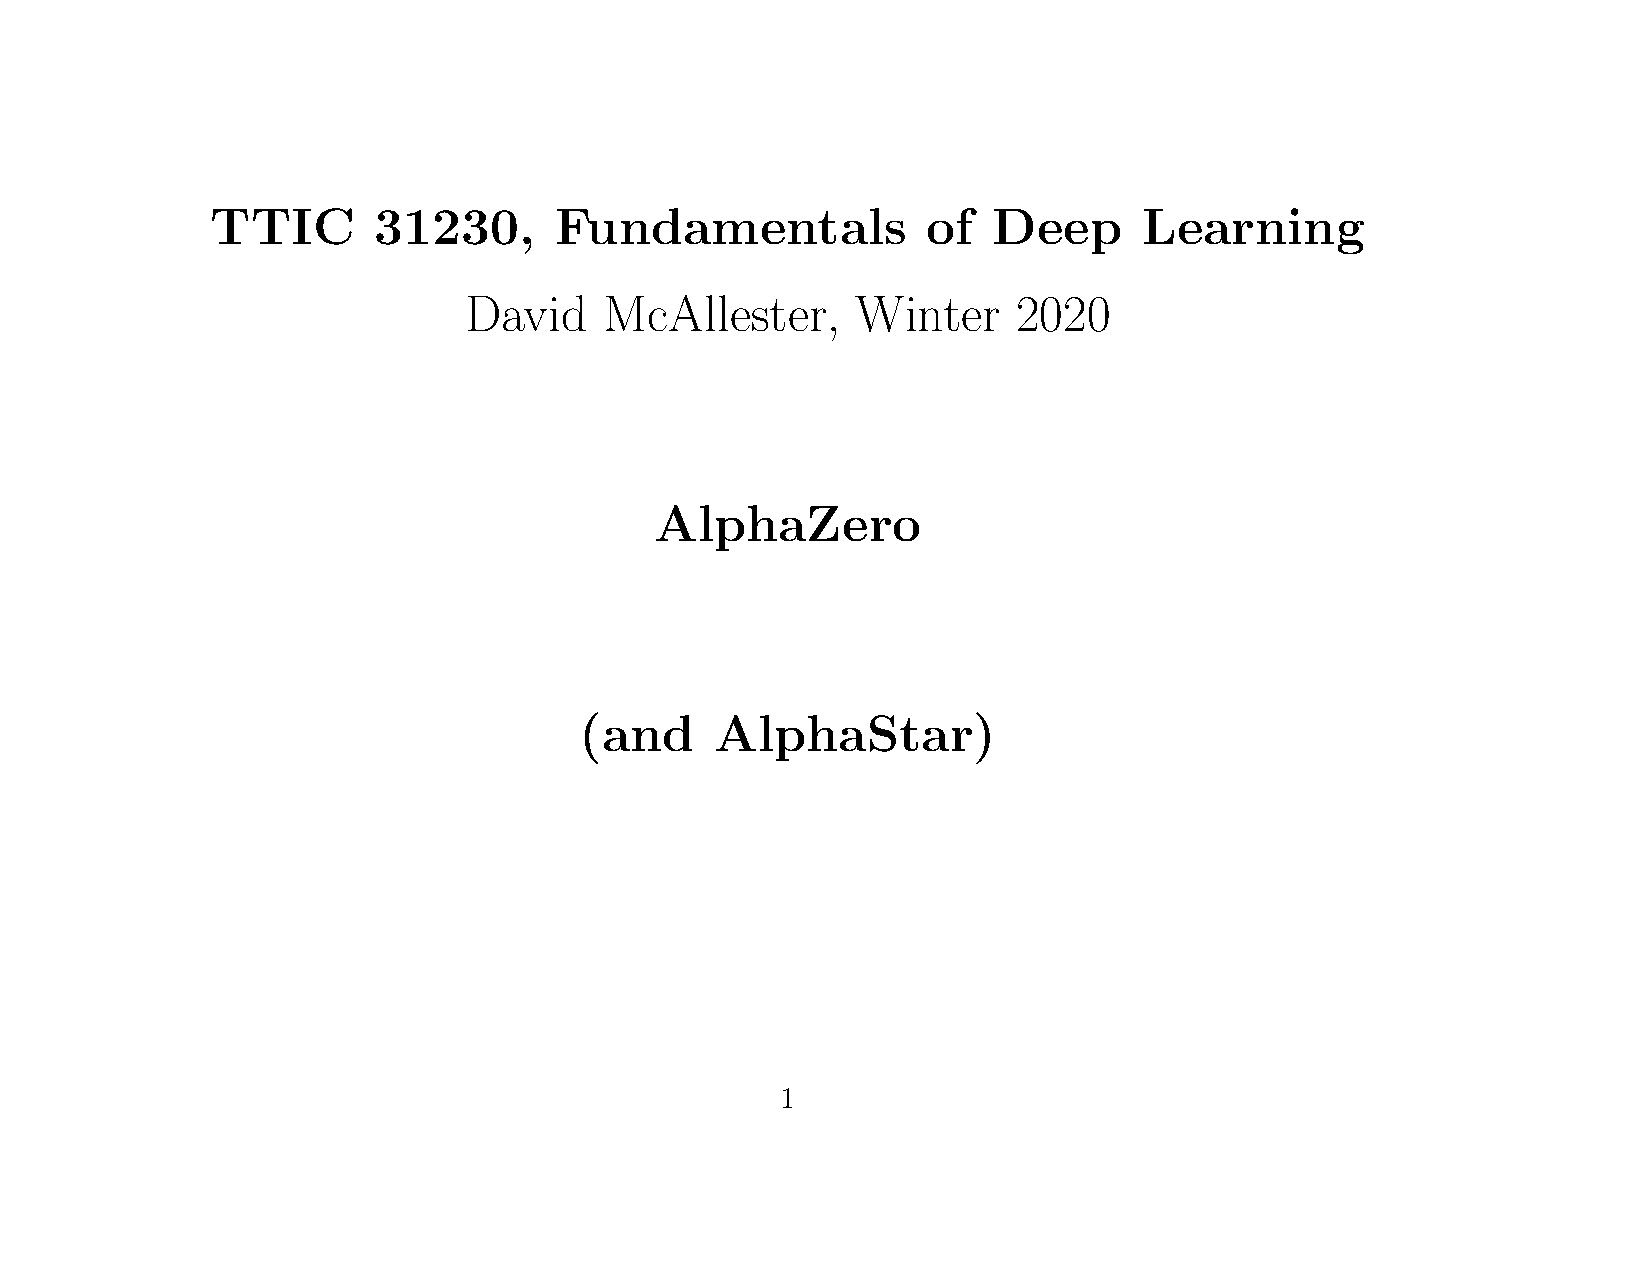
\includegraphics[width=4in]{../images/alphago}}

\slide{AlphaGo Lee (March 2016)}

\vfill
\centerline{\includegraphics[width=8in]{../images/alphagolee}}

\slide{AlphaGo Zero vs. Alphago Lee (April 2017)}

{\bf AlphaGo Lee:}

\begin{itemize}
\item Trained on both human games and self play.
  
\item Trained for Months.

\item Run on many machines with 48 TPUs for Lee Sedol match.
\end{itemize}

{\bf AlphaGo Zero:}
\begin{itemize}
\item Trained on self play only.
  
\item Trained for 3 days.

\item Run on one machine with 4 TPUs.

\item Defeated AlphaGo Lee under match conditions 100 to 0.
\end{itemize}

\slide{AlphaZero Defeats Stockfish in Chess (December 2017)}

AlphaGo Zero was a fundamental algorithmic advance for general RL.

\vfill
The general RL algorithm of AlphaZero is essentially the same as that of AlphaGo Zero.


\slide{}

\centerline{\bf Some Background}

\vfill

\slidetwo{Monte-Carlo Tree Search (MCTS)}
{Brugmann (1993)}

To estimate the value of a position (who is ahead and by how much)
run a cheap stochastic policy to generate a sequence of moves (a rollout) and see who wins.

\vfill
Select the move with the best rollout value.

\slidetwo{(One Armed) Bandit Problems}
{Robbins (1952)}

Consider a set of choices (different slot machines).

Each choice gets a stochastic reward.

\vfill
We can select a choice and get a reward as often as we like.

\vfill
We would like to determine which choice is best and also to get reward as quickly as possible.

\slidetwo{The Upper Confidence Bound (UCB) Algorithm}
{Lai and Robbins (1985)}

For each action choice (bandit) $a$, construct a confidence interval for its average reward
based on $n$ trials for that acrtion.

\vfill
$$\mu(a) \in \hat{\mu}(a) \pm 2\sigma(a)/\sqrt{n(a)}$$

\vfill
Always select

$$\argmax_a \;\; \hat{\mu}(a) + 2\sigma(a)/\sqrt{n(a)}$$

\slidetwo{The Upper Confidence Tree (UCT) Algorithm}
{Kocsis and Szepesvari (2006), Gelly and Silver (2007)}

The UCT algorithm grows a tree by running ``simulations''.

\vfill
Each simulation descends into the tree to a leaf node, expands that leaf, and returns a value.

\vfill
In the UCT algorithm each move choice at each position is treated as a bandit problem.

\vfill
We select the child (bandit) with the lowest upper bound as computed from simulations selecting that child.


\slidetwo{Bootstrapping from Game Tree Search}
{Vaness, Silver, Blair and Uther, NeurIPS 2009}

In bootstrapped tree search we do a tree search to compute a min-max value $V_{\mathrm{mm}}(s)$
using tree search with a static evaluator $V_\Phi(s)$.  We then try to fit the static value to the min-max value.

\vfill
$$\Delta \Phi = - \eta \nabla_\Phi \left(V_\Phi(s) - V_{\mathrm{mm}}(s)\right)^2$$

\vfill
This is similar to minimizing a Bellman error between $V_\Phi(s)$ and a rollout estimate of the value of $s$ but where the rollout
estimate is replaced by a min-max tree search estimate.

\slide{END}

}
\end{document}
